                %!TEX program = xelatex
\documentclass[9pt, compress]{beamer}
\usetheme[sectionpage=progressbar]{metropolis}

\usepackage{booktabs}  
\usepackage[scale=2]{ccicons}
\usepackage[T1]{fontenc}
\usepackage[utf8]{inputenc}
\usepackage{lmodern}
\usepackage{amsthm}
\usepackage{diagbox} %tabelas com barras
\usepackage{booktabs}
\usepackage{graphicx}			% Inclusão de gráficos
\usepackage[portuguese]{babel}
\newtheorem{teorema}{Teorema}


\author{\textbf{Matheus S. D'Andrea Alves}, \textbf{Uéverton dos Santos Souza} } 
\title{Coloração de Grafos$(r,\ell)$}
\subtitle{Coloração de Grafos$(r,\ell)$}
%\logo{}
\institute{\textbf{Universidade Federal Fluminense}}
\date{Julho 2018}
%\subject{}
%\setbeamercovered{transparent}
%\setbeamertemplate{navigation symbols}{}
\begin{document}
    \maketitle
    \begin{frame}{Overral}
    \centering
        \tableofcontents
    \end{frame}
    \section{O problema}
    \begin{frame}{Conceitos iniciais}
      \begin{columns}
        \begin{column}{0.5\textwidth}
          \textbf{Grafo$(r,\ell)$}
          
          Um grafo que pode ser particionado em $r$ conjuntos independentes e $\ell$ cliques.
        \end{column}
        \begin{column}{0.5\textwidth}
          \textbf{Coloração dos vértices de um grafo}
          
          Uma coloração de um grafo $G$ é uma associação de uma cor entre $k$ cores a cada vértice do grafo de forma que, dado dois vértices vizinhos em $G$ eles não compartilhem uma cor, e $k$ seja o menor número de cores possíveis a respeitar tal restrição. 
        \end{column}
      \end{columns}
    \end{frame}
    \begin{frame}[standout]
      A PERGUNTA:
      
      Quando tal problema se torna NP-Completo? 
      
      Porque?
    \end{frame}
    \section{Nossa abordagem}
    \begin{frame}{A idéia}
      Construir uma dicotomia sobre a complexidade do problema, baseando-se nos valores de $r$ e $\ell$.
      
      Analisar os resultados e investigar padrões na dificuldade do problema.
    \end{frame}
    \begin{frame}{Primeiros passos}
      Começaremos dos seguintes fatos:
      \begin{itemize}
        \item Um grafo vazio(i.e. um Grafo$(0,0)$) é 0-colorível.
        \item 
        \item 
        \item 
         \item                                                                                                                
      \end{itemize}
    \end{frame}
    \begin{frame}{Primeiros passos}
      Começaremos dos seguintes fatos:
      \begin{itemize}
        \item Um grafo vazio (i.e. um Grafo$(0,0)$) é 0-colorível.
        \item Um grafo sem arestas (i.e. um Grafo$(1,0)$) é 1-colorível.
        \item 
        \item 
         \item                                                                                                                
      \end{itemize}
    \end{frame}
    \begin{frame}{Primeiros passos}
      Começaremos dos seguintes fatos:
      \begin{itemize}
        \item Um grafo vazio (i.e. um Grafo$(0,0)$) é 0-colorível.
        \item Um grafo sem arestas (i.e. um Grafo$(1,0)$) é 1-colorível.
        \item Um grafo bipartido (i.e. um Grafo$(2,0)$) é 2-colorível.
        \item 
         \item                                                                                                                
      \end{itemize}
    \end{frame}
    \begin{frame}{Primeiros passos}
      Começaremos dos seguintes fatos:
      \begin{itemize}
        \item Um grafo vazio (i.e. um Grafo$(0,0)$) é 0-colorível.
        \item Um grafo sem arestas (i.e. um Grafo$(1,0)$) é 1-colorível.
        \item Um grafo bipartido (i.e. um Grafo$(2,0)$) é 2-colorível.
        \item Um grafo completo (i.e. um Grafo$(0,1)$) é $k-colorivel$ onde $k$ é a quantidade de vértices de G.
        \item                                                                                                               
      \end{itemize}
    \end{frame}
    \begin{frame}{Primeiros passos}
      Começaremos dos seguintes fatos:
      \begin{itemize}
        \item Um grafo vazio (i.e. um Grafo$(0,0)$) é 0-colorível.
        \item Um grafo sem arestas (i.e. um Grafo$(1,0)$) é 1-colorível.
        \item Um grafo bipartido (i.e. um Grafo$(2,0)$) é 2-colorível.
        \item Um grafo completo (i.e. um Grafo$(0,1)$) é $k-colorivel$ onde $k$ é a quantidade de vértices do grafo.
        \item Um grafo split (i.e. um Grafo$(1,1)$) é $k-colorivel$ where $k$ é a quantidade de vértices na clique máxima do grafo.
      \end{itemize}
    \end{frame}
    \begin{frame}{A mais}
      \begin{teorema}
        Coloração de Grafos(0,2) é Polinomial.
     \end{teorema}
     \begin{proof}
      Um grafo co-bipartido, é um grafo separável em 2 cliques em que todo vértice faz parte de alguma das cliques. A partir da literatura sabemos que um grafo co-bipartido é perfeito, isso é, seu número cromático é igual ao de sua clique máxima. 
      Já foi mostrado que encontrar a clique máxima em um co-bipartido é equivalente a se encontrar uma cobertura de vértices em seu complemento e portanto polinomial, ao encontrarmos a clique máxima sabemos que precisamos de seu número de vértices em cores para colorir tal grafo.
     \end{proof}
    \end{frame}
    \begin{frame}{A mais}
      \begin{teorema}
        Coloração de Grafos$(3,0)$ é Polinomial.
     \end{teorema}
     \begin{proof}
      Como sabemos que tal grafo é um Grafo(3,0) sabemos que o mesmo pode ser colorido com três cores.
      Saber se o mesmo pode ser colorido com duas ou uma cor é polinomial, portanto podemos afirmar que coloração em Grafos(3,0) é polinomial.
     \end{proof}
    \end{frame}
    \begin{frame}{A mais}
      \begin{teorema}
        Coloração de Grafos$(4,0)$ é NP-Completo.
     \end{teorema}
     \begin{proof}
      Sabemos que tal grafo é um Grafo(4,0), logo é possível o colorir com 4 cores.
      Precisamos descobrir se o mesmo pode ser colorido com menos cores; 
      Note que 3-coloração de planar é NP-Completo, e que existem subconjuntos de Grafos$(4,0)$ que são planares, logo coloração de Grafos$(4,0)$ é NP-Completo.
     \end{proof}
    \end{frame}
    \section{Primeiros resultados}
    \begin{frame}{Dicotomia parcial}
        \begin{table}[htb!]
          \center
          \begin{tabular}{l|*{7}c}
            \toprule
            \backslashbox{$r$}{$l$} & 0 & 1 & 2 & 3 & 4 & \ldots & n\\
            \midrule
            0 & \textit{P} & \textit{P} & \textit{P} & ? & ? & \ldots & ?\\
            1 & \textit{P} & \textit{P} & ? & ? & ? & \ldots & ?\\
            2 & \textit{P} & ? & ? & ? & ? & \ldots & ?\\
            3 & \textit{P} & ? & ? & ? & ? & \ldots & ?\\
            4 & \textit{NPc} & \textit{NPc} & \textit{NPc} & \textit{NPc} & \textit{NPc} & \ldots & \textit{NPc}\\
            $\vdots$ & $\vdots$ & $\vdots$ & $\vdots$ & $\vdots$ & $\vdots$ & $\ddots$ & \textit{NPc}\\
            n & \textit{NPc} & \textit{NPc} & \textit{NPc} & \textit{NPc} & \textit{NPc} & \ldots & \textit{NPc}\\
            \bottomrule
          \end{tabular}%
          \caption{Dicotomia parcial para coloração de Grafos$(r,\ell)$}
          \label{tab:tabela_part2dictrl}%
        \end{table}%
    \end{frame}
    \begin{frame}[standout]
      Como prosseguir?
    \end{frame}
    \section{A relação entre coloração e lista-coloração em Grafos$(r,\ell)$}
    \begin{frame}{A relação entre coloração e lista-coloração em Grafos$(r,\ell)$}
        \begin{teorema}
          Coloração é NP-Completo para Grafos$(r,\ell+1)$ quando lista coloração é NP-Completo para Grafo$(r,\ell)$
        \end{teorema}
    \end{frame}
    \begin{frame}{A relação entre coloração e lista-coloração em Grafos$(r,\ell)$}
        \textbf{Proof.}
        
        A prova consiste em mostrar que a solução do problema de lista coloração em um Grafo$(r,\ell)$ $G$, implica em uma solução para o problema de coloração em Grafos$(r,\ell+1)$ $H_G$.
        
        Para tanto, mostraremos que:
          \begin{itemize}
        \item Se um grafo G$(r,\ell)$ possui uma lista coloração própria então $H_G$ é k-colorível para k do tamanho da paleta $C$ (1).
		\item Se $H_G$ é k-colorível então G possui uma lista coloração própria (2).
      \end{itemize}
    \end{frame}
    \begin{frame}{A relação entre coloração e lista-coloração em Grafos$(r,\ell)$}
      \textbf{(1):}
      
      Seja $G$ um Grafo$(r,\ell)$ tal que cada vértice $v \in V(G)$ tenha uma lista de cores; 
      Cada lista tem pelo menos uma cor do seguinte conjunto: $C = \{c_1,c_2,c_3,...,c_k \}$. 
      \begin{center}
        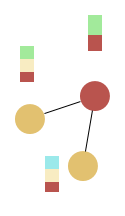
\includegraphics[scale=0.4]{../figuras/presentation-G.png}
      \end{center}
    \end{frame}
    \begin{frame}
      Seja $G$ uma instância \textbf{sim} para o problema de lista coloração, construirémos uma clique $K$, onde cada vértice $u \in V(K)$ representa uma cor de $C$.
      \begin{center}
        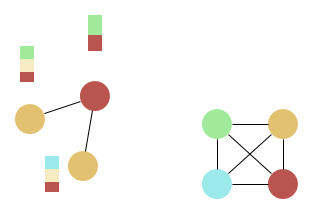
\includegraphics[scale=0.4]{../figuras/presentation-K.png}
      \end{center}
      Note tque a clique $K$ tem exatamente $k$ vértices, portanto, podemos colorir $K$ com apenas $k$ cores, sem perda de generalidade assumiremos que $u_i \in K$ será colorido com a cor $c_i$.
    \end{frame}
    \begin{frame}  
      Suponha $H_G$ $= G \cup K$, e para cada vértice $u_i \in V(K)$ e todo vértice $v_j \in V(G)$ adicione uma aresta $(u_i,v_j) $ em $H_G$ se e somente se $c_i$ não é uma cor pertencente a lista de $v_j$.
      \begin{center}
        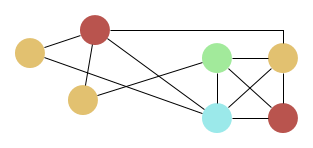
\includegraphics[scale=0.4]{../figuras/presentation-H.png}
      \end{center}   
      Usando tal coloração, a coloração de $K$ não conflita para a coloração encontrada para $G$, temos assim uma coloração para $H_G$. 
    \end{frame}
    \begin{frame}{A relação entre coloração e lista-coloração em Grafos$(r,\ell)$}
      \textbf{(2):}
      
      Sabemos que o grafo $H_G$ é um grafo$(r,\ell+1)$ e possui uma k-coloração. Onde $K$ é a clique máxima de $H_G$.
      Seja $k$ o número de vértices em $K$.
      
      Perceba que a remoção de $K$ de $H_G$ (que se tronará $G$) não afeta sua coloração, perceba que para os restantes vértices $v \in V(G)$ construímos suas listas baseando-se em seus não vizinhos em $K$ portanto a coloração adquirida em $H_G$ ainda é válida em $G$ por construção.
      
      Dessa forma mostramos que, se $H_G$ é k-colorível, $G$ é lista-colorível.
      $\qed$
    \end{frame}
    \begin{frame}{Corolários}
      Com o resultado obtido podemos afirmar que:
      \begin{itemize}
        \item Coloração em Grafos$(1,2)$ é NP-Completo.\newline Deriva da demonstração de NP-Completude para lista coloração em Split mostrado por Jensen et al. em \textit{"Generalized coloring for tree-like graphs"}.
        \item Coloração em Grafos$(2,1)$ é NP-Completo.\newline Deriva da demonstração de NP-Completude para lista coloração em bipartidos mostrado por Fellows et al. em \textit{"List Coloring and Precoloring Extension are W[1]-hard parameterized by treewidth"}.
        \item Coloração de Grafos$(0,3)$ é NP-Completo.
        \newline Deriva da demonstração de NP-Completude para lista coloração em Grafos$(0,2)$ demonstrado por Jensen et al. em \textit{"Complexity results for the optimum cost chromatic partition problem"}.
      \end{itemize}
    \end{frame}
    \begin{frame}{ Peculiaridade do Grafo$(2,1)$ }
      É trivial notar que essa classe de grafo possui um limite superior e um inferior para usa coloração ($K+1$ e $K$ respectivamente), porém apesar das restrições é NP-Completo determinar qual delas é a correta.
    \end{frame}
    \section{Resultados clássicos}
    \begin{frame}{On minimum coloring}
        Os resultados encontrado preenchem a dicotomia.
        
        \begin{table}[htb!]
          \center
          \begin{tabular}{l|*{7}c}
            \toprule
            \backslashbox{$r$}{$l$} & 0 & 1 & 2 & 3 & 4 & \ldots & n\\
            \midrule
            0 & \textit{P} & \textit{P} & \textit{P} & \textit{NPc} & \textit{NPc} & \ldots & \textit{NPc}\\
            1 & \textit{P} & \textit{P} & \textit{NPc} & \textit{NPc} & \textit{NPc} & \ldots & \textit{NPc}\\
            2 & \textit{P} & \textit{NPc} & \textit{NPc} & \textit{NPc} & \textit{NPc} & \ldots & \textit{NPc}\\
            3 & \textit{P} & \textit{NPc} & \textit{NPc} & \textit{NPc} & \textit{NPc} & \ldots & \textit{NPc}\\
            4 & \textit{NPc} & \textit{NPc} & \textit{NPc} & \textit{NPc} & \textit{NPc} & \ldots & \textit{NPc}\\
            $\vdots$ & $\vdots$ & $\vdots$ & $\vdots$ & $\vdots$ & $\vdots$ & $\ddots$ & \textit{NPc}\\
            n & \textit{NPc} & \textit{NPc} & \textit{NPc} & \textit{NPc} & \textit{NPc} & \ldots & \textit{NPc}\\
            \bottomrule
          \end{tabular}%
          \caption{Dicotomia de complexidade para coloração em Grafos$(r,\ell)$}
          \label{tab:tabela_dictrl}%
        \end{table}%
    \end{frame}
    \begin{frame}{On clique cover}
      Coloring of a Graph $G$ may be seen as \textit{Clique cover} of it's complement $G'$, impling in:
      
       \begin{table}[htb!]
          \center
          \begin{tabular}{l|*{7}c}
            \toprule
            \backslashbox{$r$}{$l$} & 0 & 1 & 2 & 3 & 4 & \ldots & n\\
            \midrule
            0 & \textit{P} & \textit{P} & \textit{P} & \textit{P} & \textit{NPc} & \ldots & \textit{NPc}\\
            1 & \textit{P} & \textit{P} & \textit{NPc} & \textit{NPc} & \textit{NPc} & \ldots & \textit{NPc}\\
            2 & \textit{P} & \textit{NPc} & \textit{NPc} & \textit{NPc} & \textit{NPc} & \ldots & \textit{NPc}\\
            3 & \textit{Npc} & \textit{NPc} & \textit{NPc} & \textit{NPc} & \textit{NPc} & \ldots & \textit{NPc}\\
            4 & \textit{NPc} & \textit{NPc} & \textit{NPc} & \textit{NPc} & \textit{NPc} & \ldots & \textit{NPc}\\
            $\vdots$ & $\vdots$ & $\vdots$ & $\vdots$ & $\vdots$ & $\vdots$ & $\ddots$ & \textit{NPc}\\
            n & \textit{NPc} & \textit{NPc} & \textit{NPc} & \textit{NPc} & \textit{NPc} & \ldots & \textit{NPc}\\
            \bottomrule
          \end{tabular}%
          \caption{Dichotomy of the clique cover problem on Graph(r,l)}
          \label{tab:tabela_dictrl}%
        \end{table}%
    \end{frame}
    \begin{frame}[standout]
      Does the Minimum vertex coloring problem has a parametrized solution for Graph(r,l)?
    \end{frame}
    \begin{frame}{Graph(2,1)}
      \large{Parametrized by the size of the smallest independent set}
      \normalsize\newline\newline
      We know the clique can be colored with k colors.
      
      We know that we can transform a minimun coloring problem into a list coloring problem.
      
      Fellows showed that the list coloring problem is w[1]-hard for bipartide graph when parametrized by the size of the smallest independent set.
      
      Minimal vertex coloring is w[1]-hard when parametrized by the smallest independet set in a Graph(2,1).
    \end{frame}
    \begin{frame}{Conclusion}
       We were sucessfull in building our foundation, answering our first question, and discovered a interesting relation between two coloring problems applied to the Graph(r,l) class.
       
       Future works:
       \begin{itemize}
         \item Why the problem behave that way?
         \item Does the Minimum vertex coloring problem has a parametrized solution for Graph(r,l)?
       \end{itemize}
     \end{frame}
     \begin{frame}[standout]
       THANK YOU!
       
       Questions?
     \end{frame}
\end{document}
